\section{Quantitative analysis of autoregressive model drift}\label{app:ddpm_drift}

Figure~\ref{fig:ddpm_drift} provides a quantitative measure of the compounding error demonstrated qualitatively in Figure~\ref{fig:denoising_trajectories} for DDPM and EDM based world models.

\begin{figure}[h!]
\begin{center}
\centerline{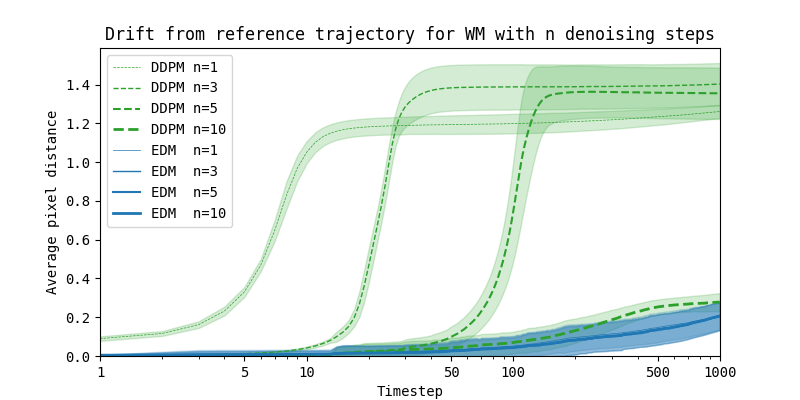
\includegraphics[width=\columnwidth]{images/drift.png}}
\caption{Average pixel drift between an imagined trajectory and the corresponding reference trajectory collected with an expert in \textit{Breakout}. The trajectories are each 1000 timesteps, starting from the same frame and following the same sequence of actions. Each line displays the average and shaded standard deviation of 400 reference trajectories held out from training data. DDPM becomes more stable with increasing number of denoising steps, but is less stable than 1-step EDM, even with 10 denoising steps. The drift we observe for EDM corresponds to differences in the imagined trajectory rather than a pathological color shift as we see in Figure 3a.}
\label{fig:ddpm_drift}
\end{center}
\end{figure}